% !TEX root = ../../STP_IoTjournal.tex
\subsection{Results \label{sec:bayArea_simResults}}
The trajectory planning for the vehicles is done using RTT algorithm, similar to that in Section \ref{sec:city_sim}-\ref{sec:city_simResults}. The resulting trajectories of vehicles are shown in Fig. \ref{fig:bayArea_d11sep5}. Once again, the vehicles remain clear of all other vehicles and reach their respective destinations. Given the separation between the scheduled times of arrival, the trajectories are predominately \textit{time-separated}, with roughly two lanes for each pair of cities (one for going from city A to city B and another for from city B to city A). A high-density of vehicles is achieved in the center since the 4 trajectories are intersecting in the center (Richmond-Oakland, Oakland-Richmond, Berkeley-San Francisco, San Francisco-Berkeley), but the STP algorithm ensures safety despite this high-density, as shown in the zoomed-in version of center at an intermediate time when a large number of vehicles are passing through the central region (Fig. \ref{fig:bayArea_d11sep5_zoomed}).  
%
\begin{figure}[H]
 \centering
\begin{subfigure}{0.5\textwidth}
  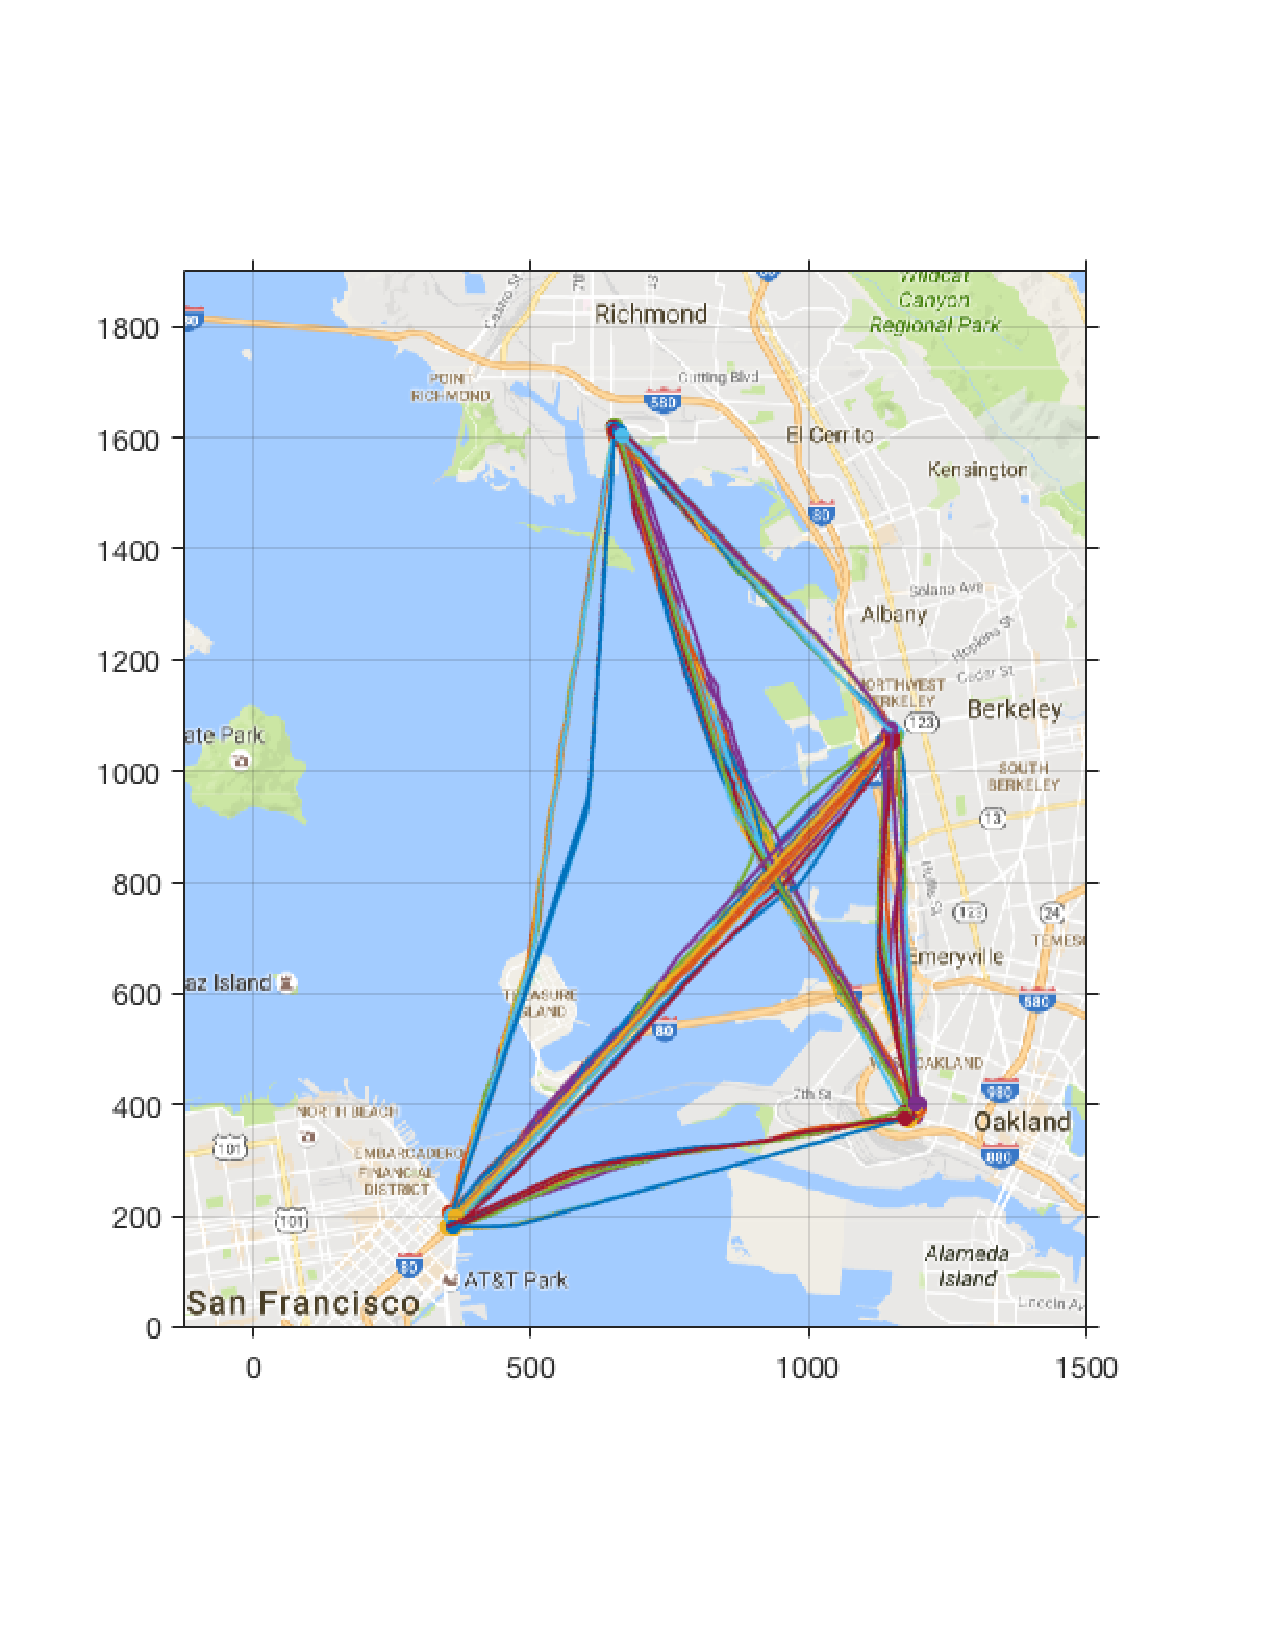
\includegraphics[width=\columnwidth]{figs/bayArea_d11sep5}
  \subcaption{}
  \label{fig:bayArea_d11sep5}
\end{subfigure}%
\begin{subfigure}{0.5\textwidth}
  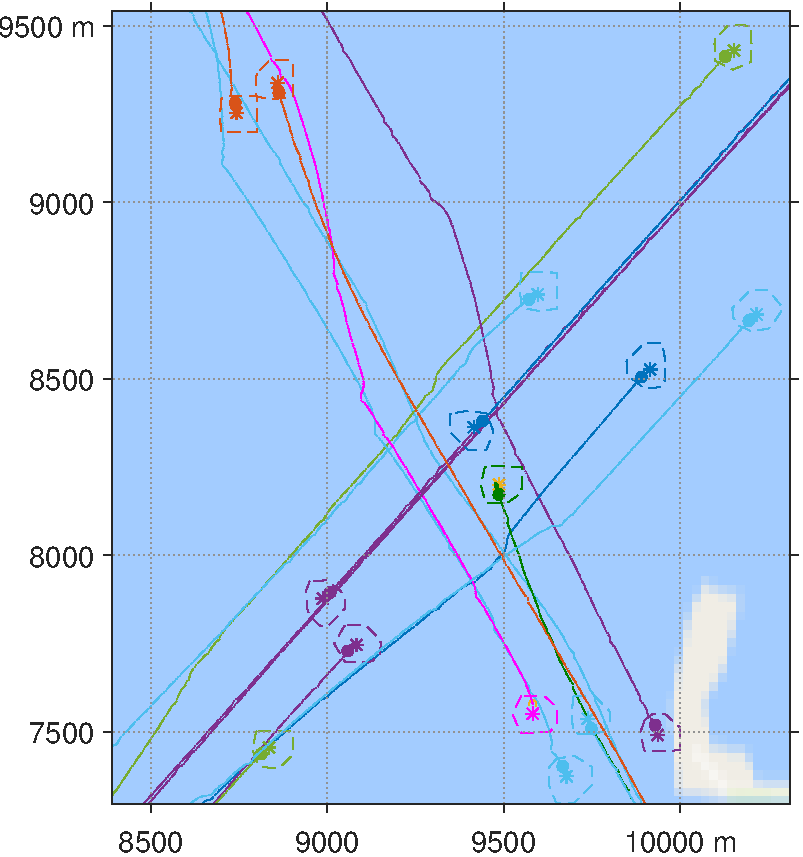
\includegraphics[width=\columnwidth]{figs/bayArea_d11sep5_zoomed}
  \subcaption{}
  \label{fig:bayArea_d11sep5_zoomed}
\end{subfigure}%
  \caption{(a) Trajectories obtained from the STP algorithm for the multi-city simulation with $d_r = 11$ m/s, $\sta_i = 5(i-1)$. (b) Zoomed-in version of the central area. A high density of vehicles is achieved at the center because of the intersection of several trajectories; however, the STP algorithm still ensures that vehicles do not enter each other's danger zones and reach their destinations.} 
  \label{fig:bayArea_d11sep5_all}
\end{figure}

Finally, we simulate the system for the case where $\sta_i = 0 ~\forall i$. As evident from Fig. \ref{fig:bayArea_d11sep0}, we get multiple lanes between each pair of cities in this case and trajectories become predominately state-separated, as we expect based on the discussion in Section \ref{sec:city_sim}-\ref{sec:city_distbEffect}.
\begin{figure}[H]
  \centering
  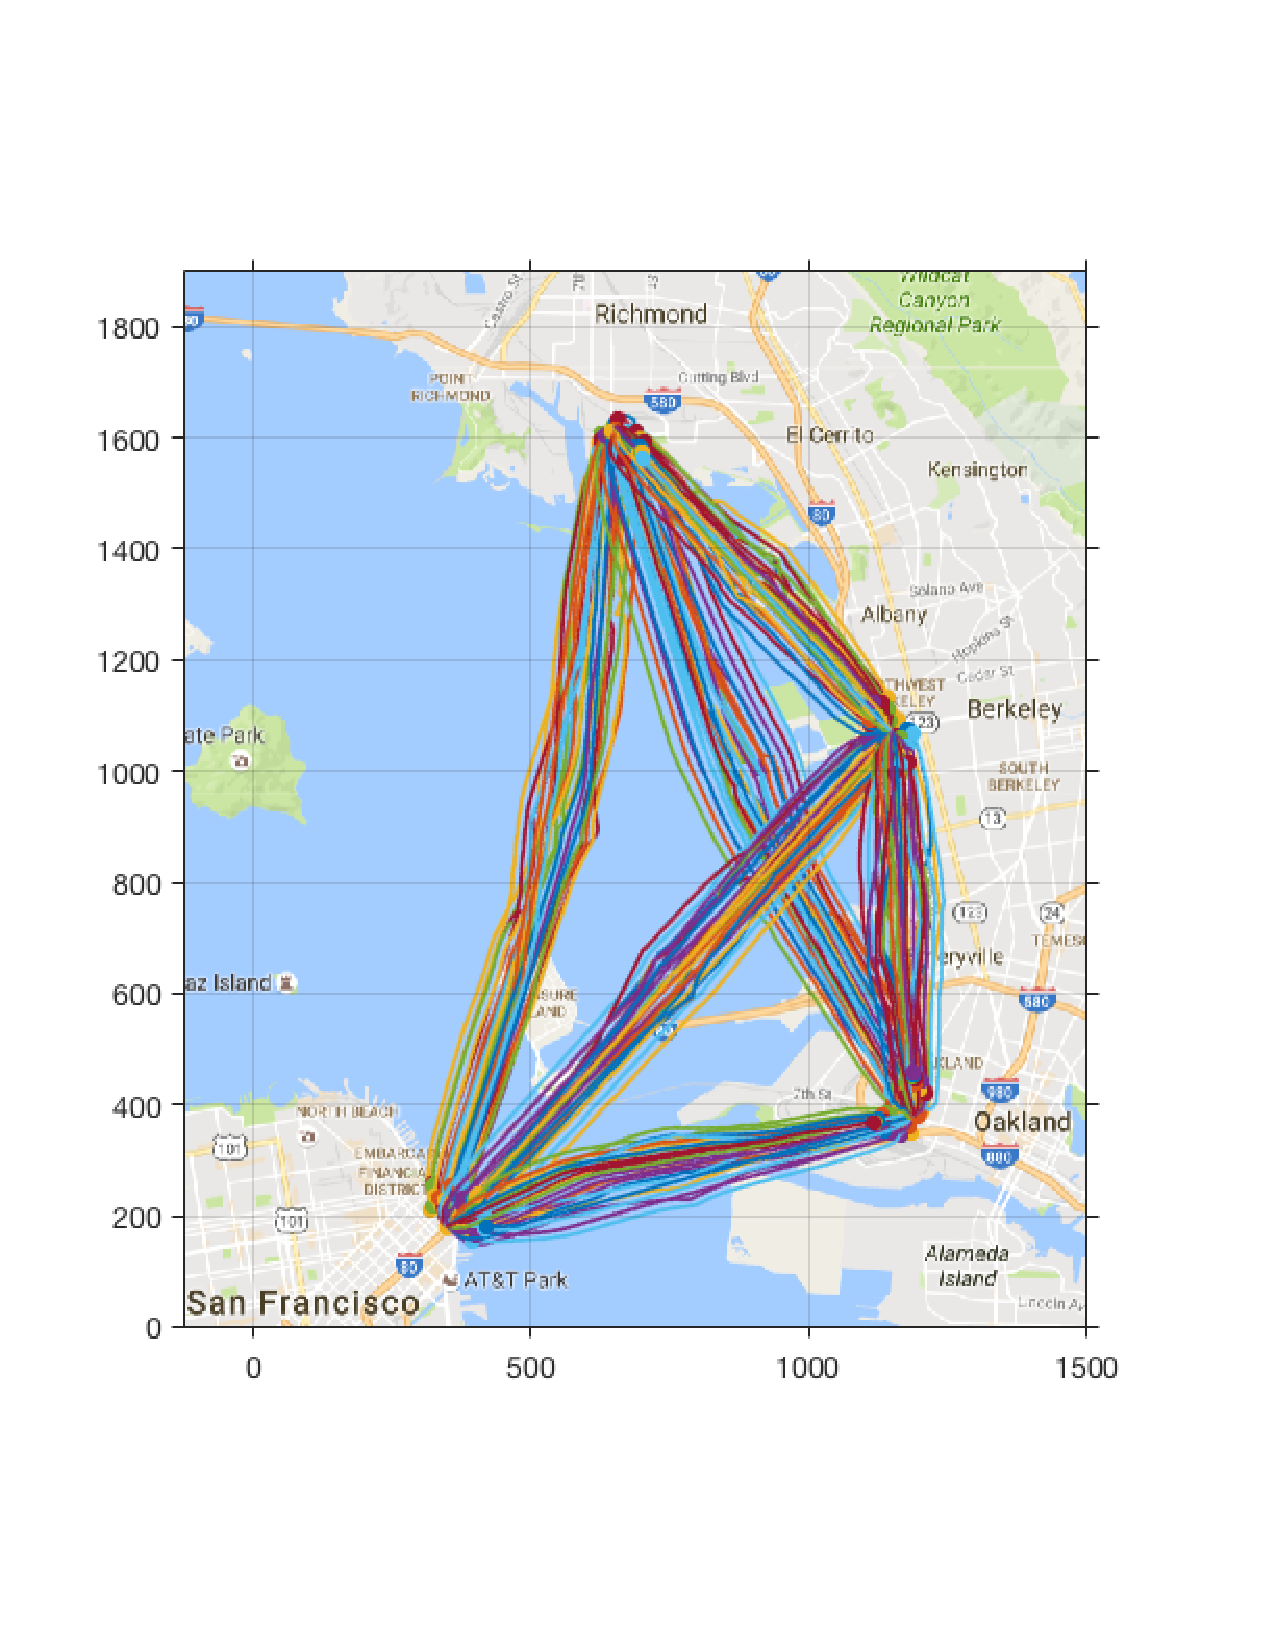
\includegraphics[width=\columnwidth]{figs/bayArea_d11sep0}
  \caption{Vehicle trajectories for $d_r = 11$ m/s, $\sta_i = 0$. Since different vehicles have same scheduled times of arrival, a multiple-lane behavior is observed between every pair of cities.} 
  \label{fig:bayArea_d11sep0}
\end{figure}

The average computation time per vehicle is 4 minutes using a CUDA implementation of the Level Set Toolbox on a desktop computer with a Core i7 5820K processor and two GeForce GTX Titan X graphics processing units. The computation time is much longer than in the previous simulation in SF because of the larger space over which planning is done. Once again all the computation is done offline and only a lookup table query is required in real-time, which can be performed very efficiently. This simulation illustrates the scalability and the potential of deploying the STP algorithm for provably safe trajectory planning for large multi-vehicle systems.